\documentclass[tikz,border=10pt]{standalone}
\begin{document}
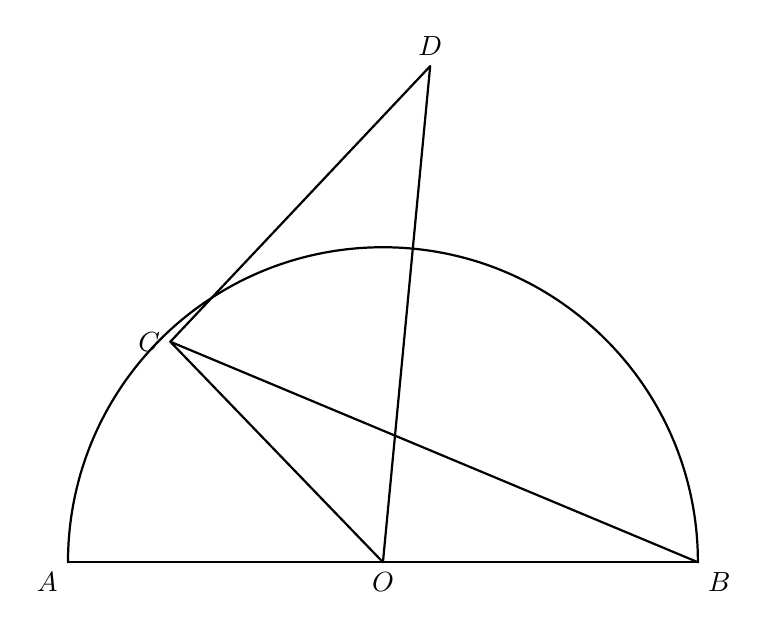
\begin{tikzpicture}[line cap=round,line join=round,thick]

\coordinate (A) at (0,0);
\coordinate (O) at (4,0);
\coordinate (B) at (8,0);
\coordinate (C) at (1.3,2.8);
\coordinate (D) at (4.6,6.3);

\draw (A) -- (B);
\draw (A) arc[start angle=180,end angle=0,radius=4];
\draw (C) -- (O);
\draw (C) -- (B);
\draw (C) -- (D);
\draw (O) -- (D);

\node[below left] at (A) {$A$};
\node[below] at (O) {$O$};
\node[below right] at (B) {$B$};
\node[left] at (C) {$C$};
\node[above] at (D) {$D$};

\end{tikzpicture}
\end{document}
